\chapter{Background Literature and Related Work}
	\label{chap:background}
	
This chapter will cover the background literature that is necessary to understand the project, including an overview of deep neural networks and general information on adversarial examples. Following that, published works on physical adversarial examples and black-box attack methods will be discussed. 

\section{Background Literature}

\subsection{Generating adversarial examples}

Generating adversarial perturbations in the white-box setting is an optimisation problem, and there is a wide variety of formulations of the problem in the literature. Szegedy \textit{et al.} \cite{szegedy2014intriguing} first defined it in the targeted setting as finding the minimum perturbation $\delta$ such that the victim model $f$ computes the desired wrong label $y^\prime$:

\begin{equation}
\label{eq:szegedy_1}
\begin{aligned}
\min_{\delta} \quad & c\|\delta\|_2\\
\textrm{s.t.} \quad & f(x + \delta) = y^\prime\\
  &x + \delta \in [0,1]^m \textrm{, m is the number of pixels in image}   \\
\end{aligned}
\end{equation}

Because equation \ref{eq:szegedy_1} is a very hard optimisation problem, Szegedy \textit{et al.} \cite{szegedy2014intriguing} use a relaxed form of the problem, where the constraint regarding the desired output is included in the objective function:

\begin{equation}
\label{eq:szegedy_2}
\begin{aligned}
\min_{\delta} \quad & c\|\delta\|_2 + L(f(x + \delta), y^\prime)\\
\textrm{s.t.} \quad& x + \delta \in [0,1]^m \textrm{, m is the number of pixels in image}   \\
\end{aligned}
\end{equation}

In equation \ref{eq:szegedy_2}, $L(\cdot)$ represents the loss function of the victim model. We want to minimise the loss in regards to the desired wrong label to increase the chance that the victim model will produce that label when the adversarial input is given.

Another paper \cite{silva_survey} defines the problem for untargeted adversarial attacks as:

\begin{equation}
\begin{aligned}
\max_{\delta} \quad & L(f(x + \delta), y)\\
\textrm{s.t.} \quad& \|\delta\|_2\leq\epsilon   \\
\end{aligned}
\end{equation}

Here, maximising the loss regarding the true label increases the chance that the model will not give that output. For targeted attacks, they define the problem as:

\begin{equation}
\label{eq:silva}
\begin{aligned}
\max_{\delta} \quad & L(f(x + \delta), y) - L(f(x + \delta), y^\prime)\\
\textrm{s.t.} \quad& \|\delta\|_2\leq\epsilon   \\
\end{aligned}
\end{equation}

In equation \ref{eq:silva}, the second term ensures that the loss function in regards to the desired wrong label is minimised.

In most papers on the subject, the optimisation problem constrains the size of the perturbation vector $\delta$ \cite{akhtar, silva_survey, tnnls_survey}. It does so by making sure that the perturbation vector's $\ell_2$ or $\ell_\infty$ norm is smaller than the maximum threshold $\epsilon$. This is to ensure that the perturbation is not too noticeable to the human eye. $\epsilon$ is often called \textbf{perturbation budget} in the literature. The $\ell_0$ norm is used by some attacks which only want to change as few pixels as possible \cite{akhtar} . 

The optimisation problem is usually solved through gradient descent. Szegedy \textit{et al.} \cite{szegedy2014intriguing} used a box constrained L-BFGS optimiser. Goodfellow \textit{et al.} \cite{fgsm} developed FGSM, a fast one-step attack method that is very popular in the literature. It calculates the gradient of the loss function of the target classifier at the given input and multiplies its sign with a constant scalar to obtain a perturbation that will change the output label.  Basic Iterative Method is an iterative version of FGSM \cite{kurakin2016adversarial}. On the other hand, generative networks can also be used instead of gradient descent optimisation to create adversarial perturbations \cite{upset_angri, zheng_black_box_GAN, advGAN}. These methods will be presented in more detail in subsection \ref{sec:generative_models}. 

You can see two examples of adversarial examples in figures \ref{fig:lbfgs} and \ref{fig:jay_adv_example}. The example in figure \ref{fig:jay_adv_example} is classified incorrectly as a mask with a confidence value of 81.8\%, while the normal image is classified correctly with a confidence value of 99.9\%.

\begin{figure}[ht]
    \centering
    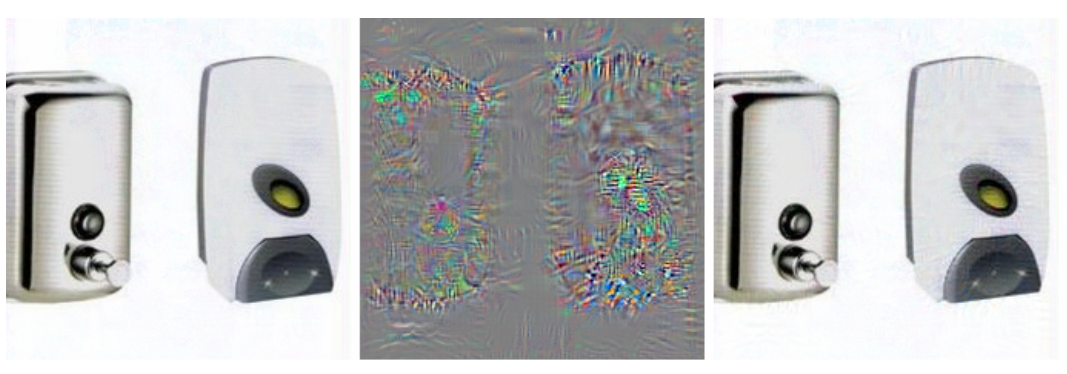
\includegraphics[width=1\textwidth]{graphics/lbfgs.PNG}
    \caption[Example of an adversarial example created by L-BFGS.]{Example of an adversarial example made by L-BFGS \cite{szegedy2014intriguing}. The left image is the original image, which is classified correctly. You can see the adversarial noise in the centre, and on the right you can see the adversarial image, which is classified as an ostrich. Image taken from \cite{szegedy2014intriguing}.}
    \label{fig:lbfgs}
\end{figure}

\begin{figure}[ht]
    \centering
    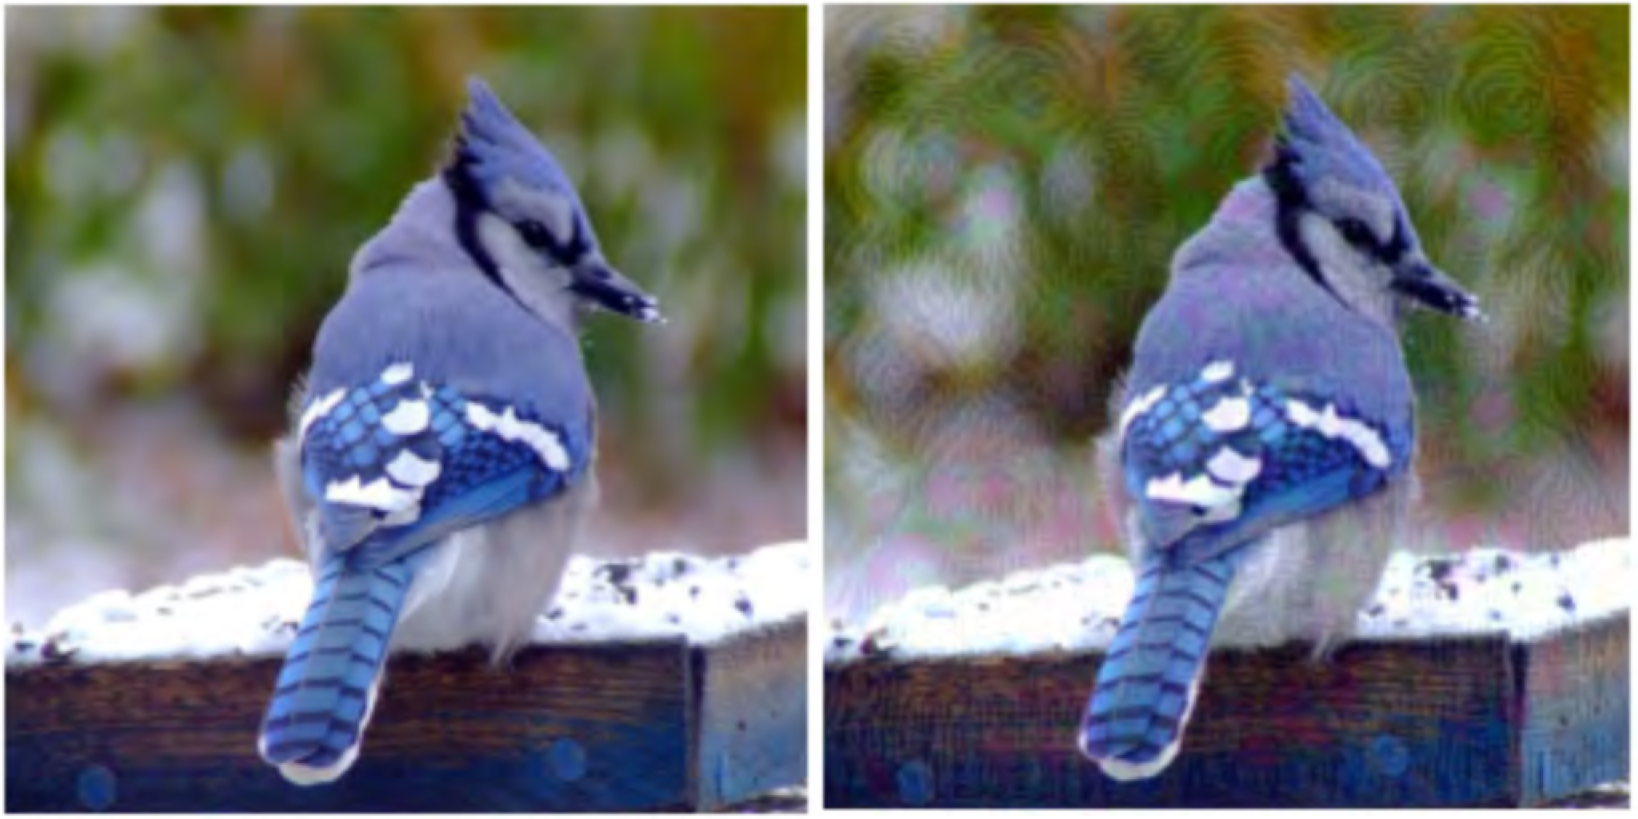
\includegraphics[width=1\textwidth]{graphics/jay_adv_example.PNG}
    \caption[Example of an adversarial example created by \cite{Moosavi-Dezfooli_2017_CVPR}.]{Example of an adversarial example created by the method in \cite{Moosavi-Dezfooli_2017_CVPR}. The left image is the original image of a jay, while the adversarial example on the right is misclassified as a mask. Images taken from \cite{akhtar}.}
    \label{fig:jay_adv_example}
\end{figure}

\subsection{Applicability of adversarial attacks}
  
Ever since the publication of \cite{szegedy2014intriguing}, most of the research has been on CNNs for object recognition tasks \cite{akhtar}. However, adversarial attacks are possible on other architectures, such as GANs \cite{kos_attacks_on_gans}, autoencoders \cite{tabacof_attacks_autoencoders}, recurrent neural networks \cite{papernot_attacks_rnns} and neural networks for semantic segmentation of an image \cite{Metzen_2017_ICCV}. Moreover, autoencoders are much more resilient against adversarial attacks \cite{tabacof_attacks_autoencoders}, and the experiments done by Tang \textit{et al.} \cite{robustart} show that Vision Transformers are more robust against adversarial attacks than CNNs.

\subsection{Transferability of adversarial examples}

Transferability-based black-box attacks succeed due to a property of adversarial examples, first discovered in \cite{szegedy2014intriguing}, that they often manage to fool victim models that are different than the model for which the adversarial example was originally made. This can happen even if the two models have different architectures. Therefore, an attacker can create adversarial perturbations for a substitute model that they control and then use them to mount an attack against another model with inaccessible parameters and loss function gradient. Dong \textit{et al.} \cite{mim} use an optimisation method with momentum to create transferability-based attacks. Meanwhile, ANGRI \cite{upset_angri} is a generative model which learns to create adversarial perturbations by using 3-4 substitute models. Similarly, Zheng \textit{et al.} \cite{zheng_black_box_GAN} train their generator against a substitute model as well.

\subsection{Taxonomy of adversarial attacks}

Silva and Najafirad \cite{silva_survey} categorises attacks based on several criteria. Depending on the \textbf{information} the attacker knows, an attack may be \textbf{white-box} or \textbf{black-box}. In the former, the attacker has full access to the architecture and parameters of the victim model, while in the latter the attacker does not have this knowledge. Dong \textit{et al.} \cite{dong2020benchmarking} further divides black-box attacks into three categories: transferability-based attacks, score-based attacks, where the attacker can query the victim model for soft-label predictions on chosen input, and then estimate the gradient, and decision-based attacks, where the attacker can only query for hard-label predictions, for which it is harder to estimate the gradient.

Attacks can also be classified depending on the \textbf{goals} of the attacker. \textbf{Untargeted} attacks only seek to make the victim model output a wrong result, whatever it may be. Meanwhile, \textbf{targeted} attacks have the goal of making the victim compute a specific wrong label. Furthermore, most attacks produce \textbf{image-specific} perturbations, which are designed to work for one specific image only. However, Moosavi-Dezfooli \textit{et al.} \cite{Moosavi-Dezfooli_2017_CVPR} discovered a method of creating \textbf{universal} adversarial noise, which induces misclassification when applied to the vast majority of images in the dataset. Finally, attacks can be categorised based on the \textbf{attack frequency}, whether the adversarial noise is generated in one step, such as in FGSM \cite{fgsm}, or in an iterative process, like in \cite{carlini2017towards}.

\subsection{Why do adversarial examples exist?}

There are varied and sometimes contradictory viewpoints in regards to why adversarial examples exist and there is no consensus. The hypothesis in Goodfellow \textit{et al.} \cite{fgsm} appears to be the more popular explanation in the literature \cite{akhtar}. This hypothesis says adversarial attacks are caused by the fact that most neural networks are too linear, which is supported by the effectiveness of the FGSM \cite{fgsm} attack method. This excessive linearity could be caused by the popular ReLU activation function, which is piece-wise linear \cite{fgsm}. In Krotov and Hopfield \cite{krotov2018dam}, experiments show that neural networks with highly non-linear activation functions can not be fooled by adversarial examples generated by models equivalent to DNNs with ReLU activation, therefore supporting the linearity hypothesis. 

On the other hand, Tanay and Griffin \cite{tanay2016boundary} contradict this and show that some linear image classifiers are not vulnerable to adversarial attacks. They hypothesize that adversarial examples exist because naturally occurring data samples exist on a subspace of the total input space and that adversarial examples exist when the classification boundary lies too close to this sub-manifold. Therefore, small perturbations manage to move the input across the decision boundary. On the other hand, their experiments show that if the decision boundary is perpendicular to this sub-manifold, the model is more robust against attacks. It is worth noting that their explanation does not totally contradict the linearity hypothesis, as the behaviour they describe is still quite linear.

On a different line of thought, Ilyas \textit{et al.} \cite{adv_examples_bugs} hypothesize that images contain subtle features that are useful for maximising the classification accuracy but are semantically meaningless in regards to the correct label. Adversarial perturbations that resemble these "non-robust" features make the victim model misclassify the adversarial examples with very high confidence.

\subsection{Defences against adversarial attacks}

Defences against adversarial attacks can be classified in the following categories \cite{silva_survey}: gradient masking, used so that the attacker can not use the loss function gradient to create adversarial examples, adversarial example detection and robust optimisation. The latter includes adversarial training, where adversarial examples labelled with the correct label are added to the training set, certified defences, where the model is proven formally to be resistant against perturbations up to a certain limit, and regularisation. The authors of the literature survey in \cite{silva_survey} put a lot of emphasis on certified defences and seem to disregard the effectiveness of adversarial training. However, Dong \textit{et al.} \cite{dong2020benchmarking} performed extensive experiments that show that adversarial training often leads to more robust models than other defences based on regularisation or certified defence.

\section{Adversarial attacks in the physical world}
    \label{sec:physical_attacks_challenges}

Most attacks, including the one in figure \ref{fig:adversarial_segmentation} on page \pageref{fig:adversarial_segmentation}, directly add the perturbations to the whole image. In a realistic setting, the attacker can not directly manipulate the pixels of the input, especially when the model takes its input from sensors. Furthermore, physical adversarial examples, whether 2D printed images or 3D objects, can have their fooling rate diminished by the angle they are viewed from, their distance from the camera, lighting conditions, the inability of the sensor to pick up the subtle adversarial perturbations, and perhaps colour printing errors \cite{kurakin2016adversarial, athalye, evtimov_road_signs}.

Kurakin \textit{et al.} \cite{kurakin2016adversarial} were among the first who investigated adversarial attacks in the physical space. They created adversarial images using FGSM \cite{fgsm}, printed them and took a picture of the printed photos using a smartphone. They then used automatic perspective transformation and cropping to transform the picture, then ran the classifier on it and compared the attack success with the original adversarial example. Over 66.67\% of adversarial examples still fooled the victim model after being printed and photographed. Therefore, it was proven that adversarial examples apply to the physical domain.

However, the photographs taken in \cite{kurakin2016adversarial} only had slight variations in terms of the camera lighting, camera distance and camera angle. Meanwhile, Lu \textit{et al.} \cite{lu_physical_experiments} did similar experiments to the ones in \cite{kurakin2016adversarial}, except they tried a wide variety of camera angles and distances, and they found that the adversarial examples were successful only when the camera was in certain positions. For example, the accuracy of the model doubled or almost tripled when the camera distance increased from 0.5m to 1.5m. Therefore, they concluded that adversarial examples may not be a serious threat to neural networks used in cyber-physical systems.

\subsection{Expectation over Transformation}
    \label{subsec:eot}

To rectify the shortcomings of adversarial attacks mentioned above, Athalye \textit{et al.} \cite{athalye} proposed the Expectation over Transformation (EOT) framework. It is designed to create adversarial examples that are effective in physical settings, and can work on 2D images, 3D rendered objects and 3D printed objects. Their key innovation is that they model transformations such as rotation, translation, perspective projection, 3D rendering or lighting in the optimisation search for the adversarial noise. 

\subsubsection{Technique}
    \label{subsubsec:eot_technique}

The authors optimise the adversarial texture $x^\prime$ in order to maximise the following objective function:

\begin{equation}
\label{eq:eot}
\begin{aligned}
\max_{x^\prime} \quad & \mathrm{E}_{t\sim T}[log P(y_{t} | t(x^\prime))] - \lambda \mathrm{E}_{t\sim T}[d(t(x^\prime), t(x))]\\
\textrm{s.t.} \quad & x \in [0, 1]^d   \\
\end{aligned}
\end{equation}

\noindent where $t(\cdot)$ is a function which simulates the various transformations, $T$ is a distribution of transformation functions, $\lambda$ is a chosen penalty constant, and $d(\cdot, \cdot)$ measures the perceptual difference between x and $x^\prime$.

While $x^\prime$ is the input that the attacker directly controls, $t(x)$ is the input seen by the neural network. In the 3D case, $x$ is a 2D texture and $t(x)$ is a 2D image of a 3D rendered object with that texture, seen from a random angle and distance. You can see an example of this in figure \ref{fig:rendering}. 

\begin{figure}[ht]
    \centering
    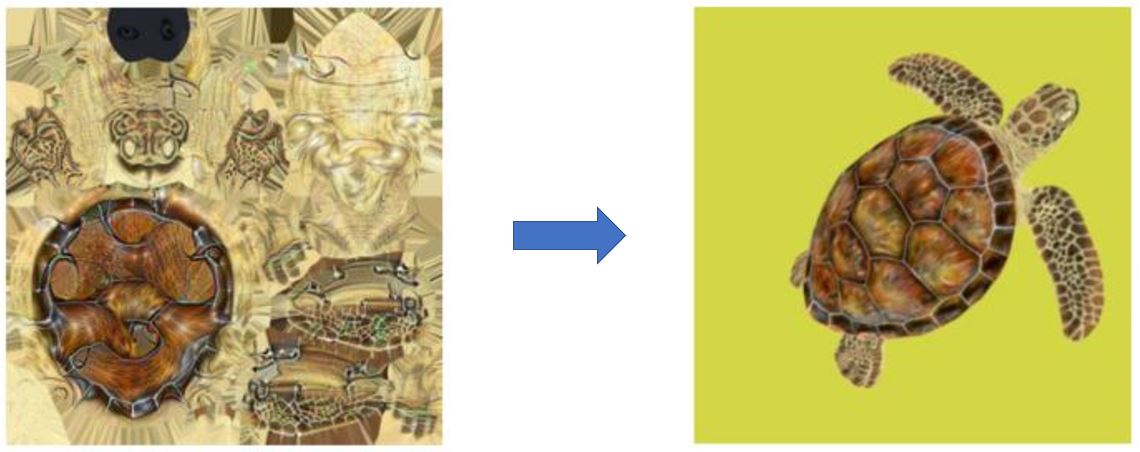
\includegraphics[width=0.8\textwidth]{graphics/rendering.JPG}
    \caption{The transformation function $t(\cdot)$ can model the rendering of a 2D texture into an image of the 3D object with a specific pose. Images are taken from \cite{athalye}.}
    \label{fig:rendering}
\end{figure}

The 3D rendering process is formally considered as a linear transformation such that $t(x) = Mx + b$. This is crucial, because EOT uses gradient descent optimisation, and therefore needs equation \ref{eq:eot} to be differentiable, including the transformation function $t(\cdot)$. The authors of \cite{athalye} claim that the coordinate map $M$ and background $b$ can be calculated for a given object pose by computing the texture-space coordinate for each corresponding on-screen pixel. $M$ and $b$ must be calculated for each new pose of the 3D model. The authors claim that they modified an existing renderer to return this information. However, they do not provide further details on how they compute $M$ and $b$, what they are exactly, nor do they mention which renderer they used. Furthermore, they do not give a link to their source code.

The first term of equation \ref{eq:eot} maximises the log probability that the neural network will classify the adversarial example as the desired target label $y_{t}$. Meanwhile, the second term minimises the distance between the adversarial example and the original input. The authors use the distance function $d(\cdot, \cdot)$ instead of $x^\prime - x$ to focus on the actual perceptual distance between the two, as the classifier sees $t(x)$ rather than $x$.

The framework leaves the choice of the distribution of transformation functions $T$ and the distance function $d(\cdot, \cdot)$ up to the user. According to the supplementary material of Athalye \textit{et al.} \cite{athalye}, the parameters for the camera distance, translation on the x and y axes, rotation of the object, lighting, and 3D printer colour error are each sampled from independent truncated uniform distributions. Camera noise is simulated by using noise drawn from a gaussian distribution.

Meanwhile, the distance metric that they used is the Euclidean distance between the projections in LAB space of $t(x)$ and $t(x^\prime)$. LAB \cite{lab} is a colour space where the Euclidean distance between two colour vectors is roughly equivalent to how different the human eye perceives those colours. The authors chose this metric so that the adversarial noise is less obvious to humans. 

In each optimisation step, the authors use the mean loss function value over a mini-batch of 40 images, each being a different transformation of the same original image. 32 of those are re-used from the previous mini-batch, while the other 8 are new images created with 8 new transformation functions drawn from the distribution $T$. The authors reuse renders as it is computationally expensive to create a new one. By using this process, they ensure that the adversarial object remains adversarial even though it is viewed from a wide variety of perspectives.

\subsubsection{Results and discussion}
    \label{subsubsec:eot_results}

To evaluate the EOT framework for generating 3D adversarial objects, the authors attack an InceptionV3 classifier \cite{inceptionv3} with 78\% accuracy on the Imagenet dataset. For the 3D rendered objects scenario, they used a dataset of 10 3D models, each representing a different class of the Imaganet dataset. For each of these models, they randomly chose 20 random target labels and then created an adversarial texture for that model and target label. 

When evaluating the 200 adversarial examples, they sample 100 random transformations from the distribution $T$ for each example and render 100 images using the adversarial texture and 100 using the original texture. The images with the normal texture had a classification accuracy of 68.8\% and were classified as the adversarial target label 1.1\% of the time. Meanwhile, the adversarial images were classified as the target label 83.4\% of the time, while only 0.01\% of these images were correctly classified.

Following that, Athalye \textit{et al.} created two 3D-printed adversarial objects, a baseball and a turtle, and found that they were classified as the target label 59\% and 82\% of the time, respectively. You can see some photos of the turtle in figure \ref{fig:3d_turtle}. Consequently, we can conclude that the EOT framework can synthesize physical 3D adversarial objects that remain highly effective when viewed from a variety of viewpoints.

Athalye \textit{et al.} \cite{athalye} provides a good high-level description of their proposed framework, and their experiment design is sound. Furthermore, their discussions offer insight into the limitations of their method. However, it lacks some critical information needed to re-create their work. As mentioned in subsection \ref{subsubsec:eot_technique}, they do not explain exactly how to get the necessary parameters to represent $t(\cdot)$ as a linear transformation, nor do they provide a link to their source code or even the data set they used. Furthermore, they do not mention what optimiser learning rate or penalty constant $\lambda$ they used or for how many steps they ran their algorithm. Finally, a step-by-step algorithm would have been useful for implementing EOT and re-creating their results.

\begin{figure}[ht]
    \centering
    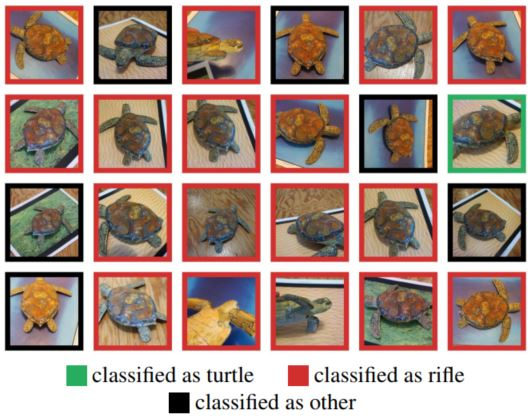
\includegraphics[width=1\textwidth]{graphics/turtle.JPG}
    \caption{A selection of photographs of the 3D adversarial turtle object. The adversarial perturbation was made for the "rifle" target label. Taken from \cite{athalye}.}
    \label{fig:3d_turtle}
\end{figure}

\subsection{Robust Physical Perturbations}

Concurrently to Athalye \textit{et al.} \cite{athalye}, Eykholt \textit{et al.} \cite{evtimov_road_signs} developed an attack for 2D physical objects, such as traffic signs, called Robust Physical Perturbations ($\textrm{RP}_2$).

\subsubsection{Technique}

In contrast with EOT \cite{athalye}, where the transformation functions from $T$ synthetically augmented the dataset by rendering the 3D object in various poses, here the authors augment it by manually taking photos of the original object from various angles and distances and in varying lighting conditions. They further use some synthetic transformations in the form of cropping and changing the image brightness to add new transformed images to the dataset. The input to $\textrm{RP}_2$ is a photo of an object taken from its front, and during the optimisation process, it draws a new sample from a distribution $X$ of images of that same object, seen under various transformations.

Moreover, because the input to $\textrm{RP}_2$ is an image of the physical 3D object rather than a 2D texture of an object, the authors use a mask $M_x$ to make sure that the adversarial perturbation $\delta$ is only applied to object itself and not to the image background. The mask is a matrix the size of the image, with a 0 for each pixel where no perturbation should be added, and 1 otherwise. 

With these changes in mind, the authors of \cite{evtimov_road_signs} define the optimisation problem in $\textrm{RP}_2$ as:

\begin{equation}
\begin{aligned}
\min_{\delta} \quad & \lambda\|M_x \cdot \delta\|_p + NPS + \mathrm{E}_{x_i\sim X}J(f_\theta(x_i + T_i(M_x \cdot \delta)), y_t)\\
\label{eq:rp2}
\end{aligned}
\end{equation}

\noindent where $NPS$ is a term for correcting printing colour errors, $J(\cdot, \cdot)$ is the loss function of the classifier represented by $f_\theta$, $y_t$ is the adversarial target label and $T_i$ is a function that transforms the perturbation to match the object in the image. If the object is seen from a 30\degree{} angle, the perturbation is rotated by 30\degree{} in 3D. The first term is for minimising the size of the perturbation, and the third term ensures that the adversarial example is misclassified.

\subsubsection{Results and discussion}
    \label{subsubsec:rp2_results}

Eykholt \textit{et al.} used $\textrm{RP}_2$ to create a poster of a road STOP sign, with perturbations applied to the whole surface of the sign. They manually took photos of the poster from a variety of distances and angles and fed them into a CNN trained on the LISA traffic sign dataset. 100\% of those photos were misclassified as the target label by the network, with an average confidence of 80.51\%. In another experiment, they created adversarial patches in the form of stickers and placed them over a STOP sign. Just like in the previous experiment, they took photos of the sign and then fed them into the LISA CNN. The attack with regular stickers had a 100\% success rate, and an attack with a sticker which looked like graffiti succeeded 66.67\% of the time. Finally, they put adversarial stickers over a real STOP sign on a street and took photos of it from a moving car. The attack success rate was 92.4\%, once more proving the effectiveness of their algorithm.

$\textrm{RP}_2$ is an interesting attack method which is capable of producing robust adversarial examples for road signs, thus endangering traffic safety. However, it is quite inconvenient. It requires the user to manually take a lot of photos and manually create the perturbation mask $M_x$. Furthermore, the authors of \cite{evtimov_road_signs} do not offer any detailed information on how the perturbation alignment function $T_i$ works, not even in the supplementary material. Finally, their approach is only applicable to flat physical surfaces, like road signs. On the other hand, EOT works for any 3D object \cite{athalye}, and could also use a mask to create adversarial patches like \cite{evtimov_road_signs} did.

\section{Generative Models for black-box attacks}
    \label{sec:generative_models}
    
\subsection{Generator-simulator model}
    \label{subsec:zheng}

Zheng \textit{et al.} \cite{zheng_black_box_GAN} proposed a generative model for creating targeted black-box adversarial examples for 2D images. Its architecture consists of two components, a generator and a simulator. The purpose of the simulator is to act as a substitute for the black-box victim model, while the generator creates adversarial noise for a given image and target label.

\subsubsection{Technique}

The simulator is trained so that it provides the same output as the victim model for a given adversarial example created by the generator:

\begin{equation}
\begin{aligned}
\min_{\theta_s} \quad & L(S(\theta_s, x + G(x, z)),V(\theta_v, x + G(x, z)))\\
\textrm{s.t.} \quad & x \in X, \|G(x, z)\|_\infty < \delta
\label{eq:simulator_loss}
\end{aligned}
\end{equation}

\noindent where the outputs predicted by the simulator and victim model are denoted by $S(\cdot,\cdot)$ and $V(\cdot,\cdot)$, respectively. $\theta_s$ and $\theta_v$ are the parameters of the simulator and victim model, respectively. The adversarial noise created by the generator for a given image $x$ and a given target label $z$ is written as $G(x,z)$. $X$ is the training set and $\delta$ is the perturbation budget. $L(\cdot,\cdot)$ represents the cross-entropy loss function. Equation \ref{eq:simulator_loss} is visualised in figure \ref{fig:zheng_simulator_loss}. It is essentially a simplified version of distillation \cite{distillation}.

\begin{figure}[ht]
    \centering
    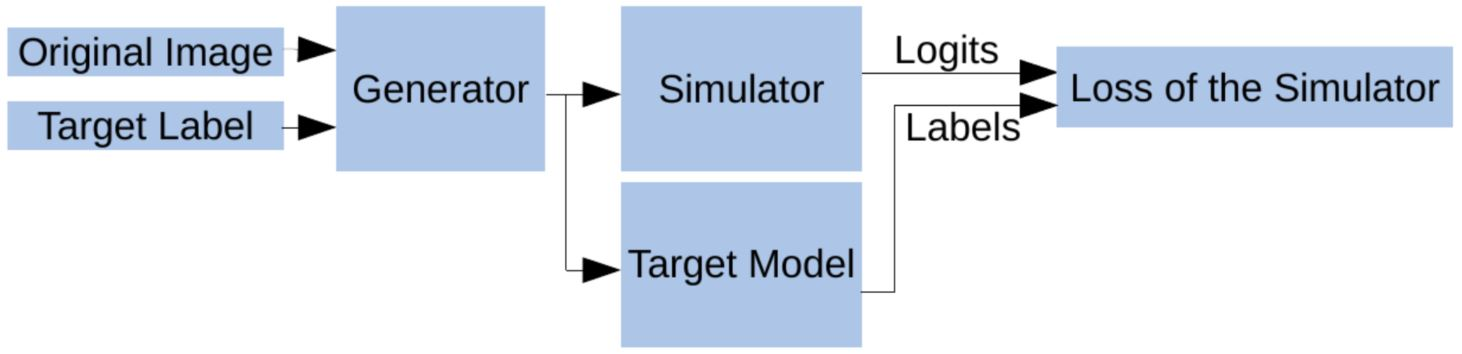
\includegraphics[width=1\textwidth]{graphics/simulator_loss.JPG}
    \caption{Computational flow of the loss function for training the simulator. Diagram taken from \cite{zheng_black_box_GAN}.}
    \label{fig:zheng_simulator_loss}
\end{figure}

Meanwhile, the generator is trained to fool the simulator such that the latter will classify the generated adversarial image with the desired wrong label $z$. Training the generator takes the following form:

\begin{equation}
\begin{aligned}
\min_{\theta_g} \quad & L(S(\theta_s, x + G(x, z)),z) + \beta\|G(x,z)\|_2\\
\textrm{s.t.} \quad & x \in X, z \in Y \setminus \{y\}\\
\label{eq:generator_loss}
\end{aligned}
\end{equation}

\noindent where $\theta_g$ is the parameter vector of the generator, $Y$ is the set of labels and $y$ is the correct label of $x$. $\beta$ is a constant for the perturbation size penalty. The first term of equation \ref{eq:generator_loss} maximises the probability that the simulator will classify the generator output as the target label, while the second term constrains the $\ell_2$ norm of the noise image vector.  Figure \ref{fig:zheng_generator_loss} visualises the generator training process.

\begin{figure}[ht]
    \centering
    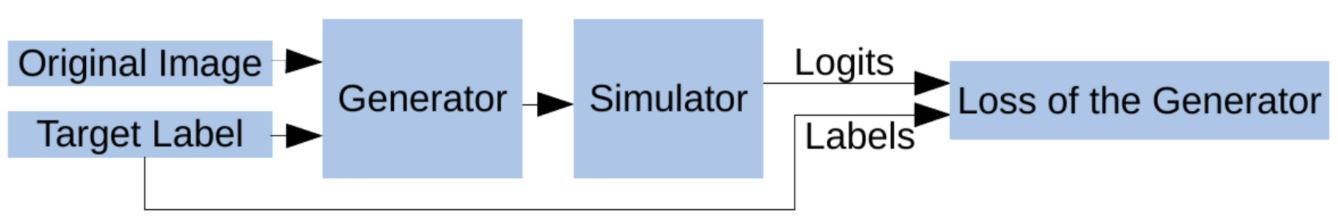
\includegraphics[width=1\textwidth]{graphics/generator_loss.JPG}
    \caption{Computational flow of the loss function for training the generator. Diagram taken from \cite{zheng_black_box_GAN}.}
    \label{fig:zheng_generator_loss}
\end{figure}

The simulator in the paper is a CNN. The proposed generator is an auto-encoder, as you can see in figure \ref{fig:zheng_generator}. The encoder takes the form of a CNN without fully connected layers or global average pooling, and its job is to encode an image as a vector in higher-dimensional latent space. 

\begin{figure}[ht]
    \centering
    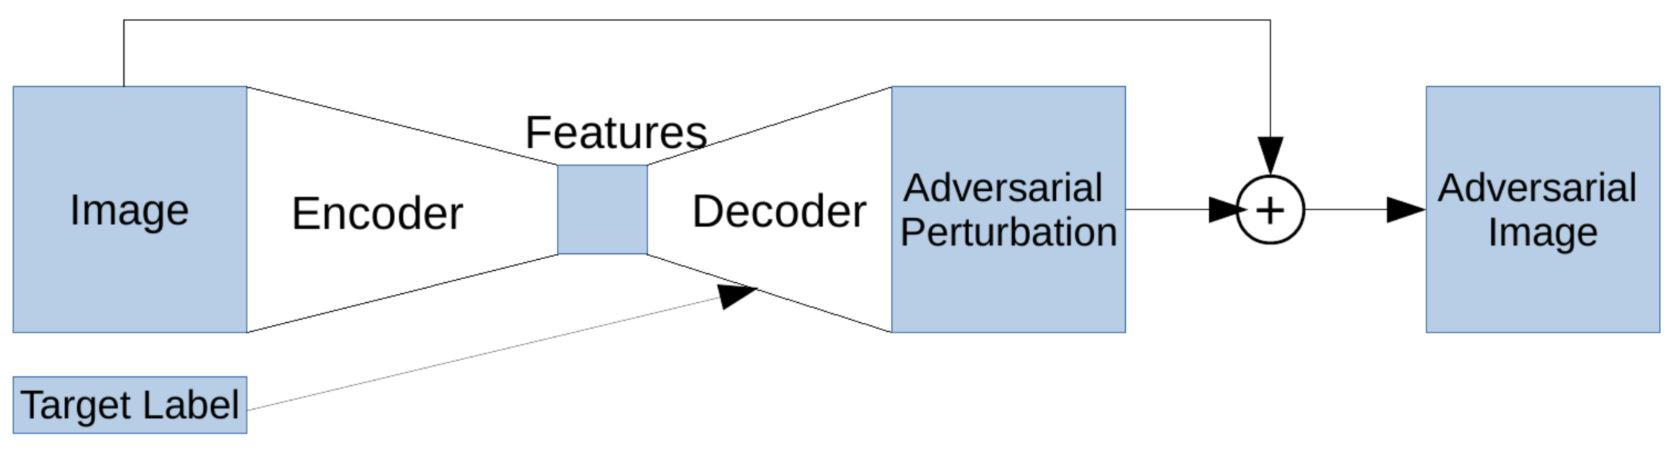
\includegraphics[width=1\textwidth]{graphics/generator.JPG}
    \caption{The autoencoder architecture of the generator in \cite{zheng_black_box_GAN}. Diagram taken from \cite{zheng_black_box_GAN}.}
    \label{fig:zheng_generator}
\end{figure}

The decoder is an ensemble of neural networks made out of transposed convolution layers, as you can see in figure \ref{fig:zheng_decoder}. It uses an ensemble because the perturbation must be designed for a given target label. The decoder has a gating sub-network inspired by Shazeer \textit{et al.} \cite{experts_mixture_gate} which learns to create a sparse weights vector based on the target label. This sub-network is just one fully connected layer with as many output neurons as there are experts. The output of the decoder is a weighted sum of the outputs of each expert model, using the weights from the gating network. Different combinations of expert models are used for different target labels, and each expert learns to focus on one or a couple of target labels.

\begin{figure}[ht]
    \centering
    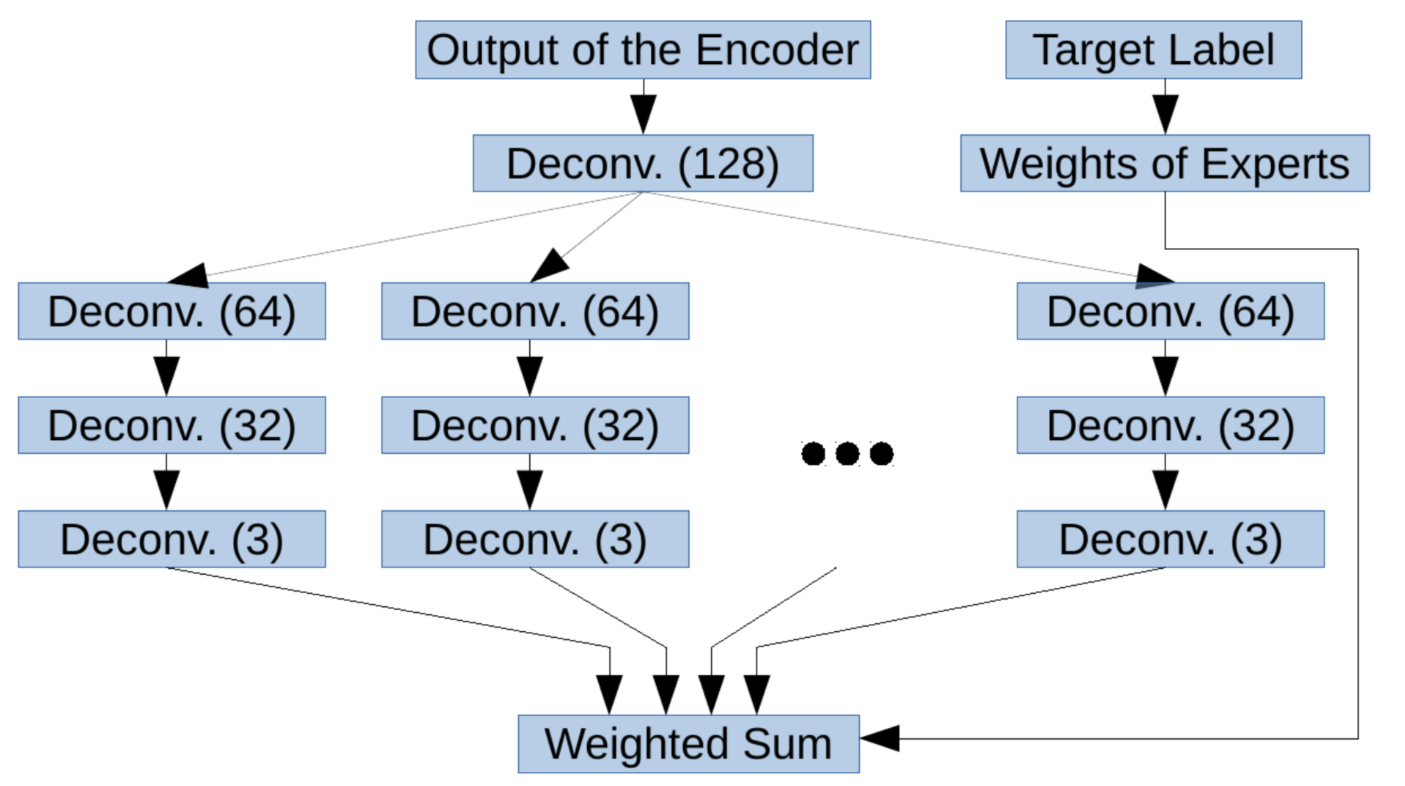
\includegraphics[width=0.8\textwidth]{graphics/decoder.PNG}
    \caption{The decoder architecture of the generator in \cite{zheng_black_box_GAN}. Diagram taken from \cite{zheng_black_box_GAN}.}
    \label{fig:zheng_decoder}
\end{figure}

The authors train the simulator and generator in alternative steps. Moreover, the authors used a number of techniques to improve results and speed-up training. Before the main training loop, they warm-up the simulator by training it on normal images. During the main loop, they also train the simulator on images with random noise, and not just with adversarial noise. Furthermore, they clip the gradients of the generator to values between -1 and 1.

\subsubsection{Results and discussion}

Zheng \textit{et al.} \cite{zheng_black_box_GAN} evaluate their model on the CIFAR-10 dataset and experiment with 4 different CNNs as simulators. These include 3 small novel CNNs, SmallNet, SimpleNet and ConcatNet, with architectures inspired by ResNet \cite{resnet}, Xception \cite{xception} and DenseNet \cite{densenet} respectively. The fourth is the Xception model \cite{xception} itself. They try all 16 possible combinations of the 4 CNNs as both simulator and victim model, with an average success rate of over 80\% across the 16 experiments and with a minimum of 63\% and a maximum of 87.3\%. Considering that all 4 CNNs had an accuracy of over 90\% on normal images, this demonstrates that the proposed technique can effectively create black-box attacks on CIFAR-10 CNNs. Moreover, it outperforms the attack success rate of the earlier generative model made by Sarkar \textit{et al.} \cite{upset_angri}. The authors repeated their experiments on CIFAR-100, where they had an attack success rate of 72.1\%.

The paper demonstrates an effective method to create a generator for black-box adversarial attacks on small images and provides plenty of details to enable someone to re-create their work. The diagrams of the model architecture are very clear, and the authors provide values for most hyper-parameters. However, they do not mention how long they trained their model, nor what learning rate, optimiser and batch size they used, and the paper does not have supplementary material. They do not provide a link to their source code either.

\subsection{AdvGAN}
    \label{subsec:AdvGAN}
    
Concurrently with Zheng \textit{et al.} \cite{zheng_black_box_GAN}, Xiao \textit{et al.} \cite{advGAN} created a generative adversarial network (GAN) \cite{gans} to create adversarial images in the black-box setting. It is similar to the former, and therefore this subsection will concentrate on the differences between the two.

\subsubsection{Technique}

AdvGAN has a generator network which produces adversarial noise and a simulator which is trained to behave like the black-box victim model, just like Zheng \textit{et al.} does. However, it also uses a discriminator, as you can see in figure \ref{fig:advgan}, where the simulator is called a "distilled black-box". 

\begin{figure}[ht]
    \centering
    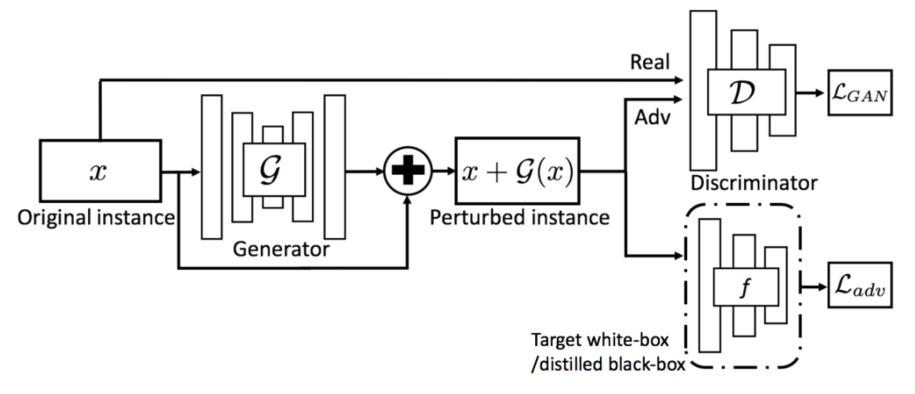
\includegraphics[width=0.8\textwidth]{graphics/advgan.PNG}
    \caption{High-level overview of AdvGAN. Diagram taken from \cite{advGAN}.}
    \label{fig:advgan}
\end{figure}

Unlike in \cite{zheng_black_box_GAN}, the generator trains to fool the discriminator into thinking adversarial images are normal images, while also training to fool the simulator into classifying the adversarial images as the desired target label. Meanwhile, the discriminator trains to tell if an image contains noise made by the generator. The generator training against the discriminator ensures that the adversarial noise is hard to distinguish. The noise is further constrained by a hinge loss:

\begin{equation}
\begin{aligned}
\mathrm{L}_\textrm{hinge} = \mathrm{E}_x max(0, \|G(x)\|_2 - c)\\
\label{eq:advgan_hing_loss}
\end{aligned}
\end{equation}

which adds a penalty if the Euclidean length of the noise vector is under $c$, while Zheng \textit{et al.} simply used an $\ell_2$ penalty term.

The simulator is trained to behave like the victim model using distillation \cite{distillation}. After every step of training the generator and discriminator, the simulator performs a training step with both normal and adversarial images as input. On the other hand, Zheng \textit{et al.} \cite{zheng_black_box_GAN} only do so with adversarial images and trains the simulator on normal images only during the initial warm-up phase.

The discriminator of AdvGAN is a CNN which performs binary classification on patches of the input image and then averages the patch predictions to determine if the whole image is adversarial. The generator is an auto-encoder where the encoder is made up of convolutional layers, while the decoder is made of transposed convolutions. Unlike in the generator of Zheng \textit{et al.}, AdvGAN has pairs of encoder and decoder layers with residual connections between them, as U-Net does \cite{unet}. Finally, the generator of AdvGAN does not make use of a mixture-of-experts in its decoder, and therefore it can not generate perturbations for all target labels and must be re-trained for each target label. This is in contrast with the generator in subsection \ref{subsec:zheng}, which could generate adversarial examples for any target label.

\subsubsection{Results and discussion}

The authors evaluate AdvGAN against ResNet-32 and Wide ResNet-34 \cite{resnet} models trained on CIFAR-10, and in the black-box setting the targeted attack has a success rate of 78.5\% and 81.8\%, respectively. Moreover, it achieved an attack success rate of 92.76\% in the black-box setting of the MadryLab challenge \cite{madrylab}. Finally, the authors claim that they managed to create adversarial noise for 100 high-resolution ImageNet-like images against an InceptionV3 model \cite{inceptionv3} with a 100\% attack success rate.

Xiao \textit{et al.} created a powerful generative network for targeted black-box attacks, and the paper provides a lot of detail on the overview of the model and on how it is trained. Moreover, it performs a wide range of experiments, with both white-box and black-box settings, as well as attacking models with defences against adversarial attacks. However, they do not provide detailed information on the exact architecture they used for the discriminator and generator, they just say "adopt similar architectures for generator and discriminator with image-to-image translation literature" then cite two papers. They do not provide source code or supplementary material either. However, the largest downside of their model is that it must be trained for each individual target label.

Furthermore, their claim of a 100\% attack success rate on high-resolution images is odd, as they do not mention how they adapted their architecture for larger input, and it makes no sense how the attack was even more successful than against simpler models on CIFAR-10. The example Imagenet adversarial images in the paper look identical to the normal images, too.
